\documentclass[12pt,a4paper]{article}

% ── Packages ──
\usepackage[utf8]{inputenc}
\usepackage[T1]{fontenc}
\usepackage{lmodern}
\usepackage[margin=2.5cm]{geometry}
\usepackage{amsmath,amssymb}
\usepackage{graphicx}
\usepackage{booktabs}
\usepackage{hyperref}
\usepackage{xcolor}
\usepackage{enumitem}
\usepackage{listings}
\usepackage{float}
\usepackage{caption}
\usepackage{fancyhdr}
\usepackage{titlesec}
\setlength{\parskip}{6pt plus 2pt minus 1pt}
\setlength{\parindent}{0pt}

% ── Styling ──
\hypersetup{
    colorlinks=true,
    linkcolor={blue!60!black},
    citecolor={blue!60!black},
    urlcolor={blue!60!black}
}

\lstset{
    basicstyle=\ttfamily\small,
    backgroundcolor=\color{gray!10},
    frame=single,
    rulecolor=\color{gray!40},
    breaklines=true,
    showstringspaces=false,
    keywordstyle=\color{blue!70!black},
    commentstyle=\color{green!50!black},
    stringstyle=\color{red!60!black},
    language=Python
}

\pagestyle{fancy}
\fancyhf{}
\fancyhead[L]{\small SLAM-Based Mapping Robot}
\fancyhead[R]{\small MSc Artificial Intelligence}
\fancyfoot[C]{\thepage}

\titleformat{\section}{\Large\bfseries}{\thesection}{1em}{}
\titleformat{\subsection}{\large\bfseries}{\thesubsection}{1em}{}
\titleformat{\subsubsection}{\normalsize\bfseries}{\thesubsubsection}{1em}{}

% ══════════════════════════════════════════════════════════════
\begin{document}

% ── Title Page ──
\begin{titlepage}
\centering
\vspace*{3cm}
{\Huge\bfseries SLAM-Based Mapping Robot\\[0.4cm]}
{\Large Perception \& Kinematics}\\[2cm]
{\large\textbf{Name:} Kinyua Seaman}\\[0.3cm]
{\large\textbf{Module:} Robotics --- MSc Artificial Intelligence}\\[0.5cm]
{\large\textbf{Date:} May 2026}\\[0.5cm]
{\large\textbf{Project Type:} Simulation-Based Coursework}\\[3cm]
\vfill
\end{titlepage}

\tableofcontents
\newpage

% ══════════════════════════════════════════════════════════════
\section{Introduction}

Simultaneous Localisation and Mapping (SLAM) is a fundamental problem in autonomous robotics: a mobile agent must incrementally construct a map of an unknown environment while simultaneously tracking its own position within that map. The problem is circular---accurate mapping requires a good pose estimate, yet accurate localisation requires a good map---and has been studied extensively since the seminal work of Smith, Self and Cheeseman (1990) and the probabilistic formulation by Thrun, Burgard and Fox (2005).

This project implements a \textbf{custom, from-scratch 2D SLAM simulation} in Python that explicitly models:

\begin{enumerate}
    \item \textbf{Differential-drive kinematics} with stochastic odometry noise,
    \item \textbf{2D LiDAR ray-casting} with configurable Gaussian sensor noise, and
    \item \textbf{Log-odds occupancy grid mapping} using Bresenham's line algorithm for efficient ray-to-cell projection.
\end{enumerate}

The simulation was developed without ROS/Gazebo, requiring every subsystem---physics, sensing, mapping, and visualisation---to be hand-coded, thereby deepening engagement with the underlying mathematics.

\subsection{Aims and Learning Outcomes}

\begin{table}[H]
\centering
\begin{tabular}{@{}p{4.5cm}p{9cm}@{}}
\toprule
\textbf{Learning Outcome} & \textbf{How Addressed} \\
\midrule
Probabilistic Robotics & Log-odds occupancy grid; Gaussian motion \& observation noise models \\
Sensor Fusion & Noisy odometry pose fused with LiDAR depth scans to infer grid state \\
Coordinate Frame Management & Local robot frame (LiDAR bearings) $\leftrightarrow$ global map frame (occupancy grid indices) \\
Motion Planning (basic) & Proportional waypoint-following controller \\
\bottomrule
\end{tabular}
\end{table}

% ══════════════════════════════════════════════════════════════
\section{Theoretical Background}

\subsection{Differential-Drive Kinematics}

The robot is modelled as a differential-drive platform governed by the velocity motion model (Thrun et al., 2005, Ch.~5). Given linear velocity~\(v\) and angular velocity~\(\omega\), the continuous-time kinematic equations in the global frame are:

\begin{equation}
    \dot{x} = v \cos\theta, \qquad \dot{y} = v \sin\theta, \qquad \dot{\theta} = \omega
\end{equation}

For the discrete time step \(\Delta t\), two cases are handled:

\paragraph{Pure translation (\(\omega = 0\)):} Euler integration is applied directly.

\paragraph{Arc motion (\(\omega \neq 0\)):} The exact closed-form arc equations are used:

\begin{align}
    x_{t+1} &= x_t - \frac{v}{\omega}\sin\theta_t + \frac{v}{\omega}\sin(\theta_t + \omega\Delta t) \\[6pt]
    y_{t+1} &= y_t + \frac{v}{\omega}\cos\theta_t - \frac{v}{\omega}\cos(\theta_t + \omega\Delta t) \\[6pt]
    \theta_{t+1} &= \theta_t + \omega\Delta t
\end{align}

This closed-form integration is more accurate than na\"ive Euler for non-zero curvature and avoids the systematic drift that plagues first-order approximations over long trajectories.

\subsection{Odometry Noise Model}

Noisy odometry is generated by corrupting the commanded velocities:

\begin{align}
    \hat{v} &= v + \varepsilon_v, \qquad \varepsilon_v \sim \mathcal{N}\!\left(0,\; \alpha_1 v^2 + \alpha_2 \omega^2\right) \\[6pt]
    \hat{\omega} &= \omega + \varepsilon_\omega, \qquad \varepsilon_\omega \sim \mathcal{N}\!\left(0,\; \alpha_3 v^2 + \alpha_4 \omega^2\right)
\end{align}

The noise parameters \(\alpha_1 \ldots \alpha_4\) control the velocity-dependent covariance structure. This is the standard four-parameter model from Thrun et al.\ (2005, Table~5.6), ensuring that noise scales realistically with commanded motion---faster speeds and sharper turns produce proportionally larger odometry errors. A small constant (\(10^{-6}\)) is added inside the square root for numerical stability when both velocities are near zero.

\subsection{LiDAR Sensor Simulation}

The simulated 2D LiDAR casts \(N = 72\) rays uniformly over a full \(2\pi\) field of view. Each ray is traced incrementally through the occupancy grid at half-resolution step size (\(0.5\,\text{m}\)) until either:

\begin{itemize}
    \item An \textbf{occupied cell is hit}: the distance is recorded plus additive Gaussian noise \(\varepsilon_d \sim \mathcal{N}(0, \sigma_d)\), or
    \item The \textbf{maximum range} (\(15\,\text{m}\)) is reached: a max-range reading is returned.
\end{itemize}

\textbf{Note:} The ray-casting operates in the \textbf{global frame} using the robot's \emph{true} pose, not the estimated pose. This is physically correct: the sensor measures the real world. The noisy estimated pose is used only when integrating these readings into the map---faithfully modelling the effect of localisation error on map quality.

\subsection{Log-Odds Occupancy Grid Mapping}

The occupancy grid represents the environment as a discretised 2D array where each cell \(m_{i,j}\) stores the log-odds of occupancy:

\begin{equation}
    l_{i,j} = \log\frac{P(m_{i,j} = 1 \mid z_{1:t})}{P(m_{i,j} = 0 \mid z_{1:t})}
\end{equation}

Under a static-world assumption and conditional independence of observations given the map, the Bayesian update in log-odds form reduces to a simple additive update (avoiding costly multiplications and normalisations):

\begin{equation}
    l_{i,j}^{\,t} = l_{i,j}^{\,t-1} + l_{\text{inv}} - l_0
\end{equation}

\begin{table}[H]
\centering
\begin{tabular}{@{}ccp{7.5cm}@{}}
\toprule
\textbf{Symbol} & \textbf{Value} & \textbf{Meaning} \\
\midrule
\(l_{\text{occ}}\)  & \(\log\frac{0.7}{0.3} \approx 0.847\) & Inverse-sensor log-odds for occupied cells \\[4pt]
\(l_{\text{free}}\) & \(\log\frac{0.3}{0.7} \approx -0.847\) & Inverse-sensor log-odds for free cells \\[4pt]
\(l_0\)             & \(0.0\) & Prior log-odds (maximum uncertainty) \\
\bottomrule
\end{tabular}
\end{table}

The grid is initialised to \(l_0 = 0\) (50\% prior probability). Repeated observations drive cells towards strong occupied or free beliefs. The final probability is recovered via the logistic function:

\begin{equation}
    P(m_{i,j} = 1) = 1 - \frac{1}{1 + \exp(l_{i,j})}
\end{equation}

\subsection{Bresenham's Line Algorithm}

To determine which grid cells each LiDAR ray passes through, the implementation uses \textbf{Bresenham's line algorithm}---an integer-arithmetic rasterisation method that enumerates all cells along a line from the sensor origin to the ray endpoint. All intermediate cells are marked as free (\(+l_{\text{free}}\)) and the terminal cell (if a hit occurred) is marked as occupied (\(+l_{\text{occ}}\)). This is computationally efficient (no floating-point divisions per step) and avoids the aliasing artifacts that simpler stepping methods can introduce.

% ══════════════════════════════════════════════════════════════
\section{System Architecture}

The project follows a modular, object-oriented design with clear separation of concerns. The data flow is:

\begin{center}
\fbox{\texttt{main.py}} $\longrightarrow$
\fbox{\texttt{Environment}} $\xrightarrow{\text{true pose} \to \text{LiDAR scan}}$
\fbox{\texttt{main.py}} $\xrightarrow{\text{est.\ pose + scan}}$
\fbox{\texttt{OccupancyGridMap}}
\end{center}

\vspace{0.3cm}
\begin{center}
\fbox{\texttt{main.py}} $\longrightarrow$
\fbox{\texttt{Robot}} $\xrightarrow{\text{noisy odometry}}$
\fbox{\texttt{main.py}}
\end{center}

\subsection{Module Descriptions}

\subsubsection{\texttt{environment.py} --- World \& Sensor}

\begin{table}[H]
\centering
\begin{tabular}{@{}p{3.5cm}p{10cm}@{}}
\toprule
\textbf{Responsibility} & \textbf{Details} \\
\midrule
Grid construction & 50$\times$50\,m world at 1\,m resolution $\to$ 50$\times$50 cell array \\
Obstacle generation & Outer boundary walls + 3 fixed inner walls + 5 random rectangular blocks \\
LiDAR simulation & \texttt{get\_lidar\_scan}: ray-casting with configurable max range, ray count, FOV, and noise \\
\bottomrule
\end{tabular}
\end{table}

\subsubsection{\texttt{robot.py} --- Kinematics \& Odometry}

\begin{table}[H]
\centering
\begin{tabular}{@{}p{3.5cm}p{10cm}@{}}
\toprule
\textbf{Responsibility} & \textbf{Details} \\
\midrule
True motion & Exact arc-based differential-drive update \\
Noisy odometry & Velocity-dependent Gaussian corruption (\(\alpha_1\)--\(\alpha_4\)) \\
Path tracking & Maintains separate \texttt{true\_path} and \texttt{estimated\_path} histories \\
Visualisation helper & \texttt{plot\_robot}: renders a circle + heading line \\
\bottomrule
\end{tabular}
\end{table}

\subsubsection{\texttt{slam.py} --- Occupancy Grid Mapping}

\begin{table}[H]
\centering
\begin{tabular}{@{}p{3.5cm}p{10cm}@{}}
\toprule
\textbf{Responsibility} & \textbf{Details} \\
\midrule
Log-odds grid & Initialised to 0 (uniform prior) \\
Bayesian update & \texttt{update}: iterates over LiDAR rays, applies Bresenham, updates cells \\
Bresenham rasterisation & \texttt{bresenham}: generator yielding (x, y) integer grid coordinates \\
Probability conversion & \texttt{get\_map\_probabilities}: logistic transform for visualisation \\
\bottomrule
\end{tabular}
\end{table}

\subsubsection{\texttt{main.py} --- Simulation Orchestrator}

\begin{table}[H]
\centering
\begin{tabular}{@{}p{3.5cm}p{10cm}@{}}
\toprule
\textbf{Responsibility} & \textbf{Details} \\
\midrule
Waypoint navigation & 8 predefined waypoints with proportional heading controller \\
Simulation loop & Up to 1500 steps at \(\Delta t = 0.1\,\text{s}\) \\
Visualisation & Dual-panel matplotlib figure saved every 50 steps \\
Evaluation & Terminal MSE between true and estimated (x, y) positions \\
\bottomrule
\end{tabular}
\end{table}

\subsubsection{\texttt{visualization.html} --- Interactive Web Demo}

A standalone HTML/Canvas/JavaScript re-implementation of the full pipeline (environment, robot, occupancy grid, Bresenham) with real-time rendering and user-adjustable sliders for linear speed, angular speed, and sensor noise.

% ══════════════════════════════════════════════════════════════
\section{Implementation Details}

\subsection{Waypoint Navigation Controller}

The robot is driven by a simple \textbf{proportional controller}:

\begin{lstlisting}
target_theta = np.arctan2(dy, dx)
angle_diff = robot.normalize_angle(target_theta - rtheta)

v = min(2.0, distance) if abs(angle_diff) < np.pi/4 else 0.0
w = max(-1.0, min(1.0, angle_diff * 2.0))
\end{lstlisting}

Key design choices:
\begin{itemize}
    \item \textbf{Heading-gated linear velocity:} The robot only drives forward when the heading error is within \(\pm 45^\circ\), preventing large lateral drift during turns.
    \item \textbf{Clamped angular velocity:} \(\omega \in [-1, 1]\,\text{rad/s}\) prevents physically unrealistic instantaneous rotation.
    \item \textbf{Speed proportional to distance:} \(v = \min(2.0, d)\) provides natural deceleration as waypoints are approached, reducing overshoot.
\end{itemize}

\subsection{Sensor--Map Integration}

A critical architectural decision is the separation of sensing and mapping:

\begin{lstlisting}
# LiDAR scan from TRUE pose (physically correct)
rel_angles, distances = env.get_lidar_scan(robot.true_pose, num_rays=72)

# Map update using ESTIMATED pose (simulates real-world SLAM)
slam.update(robot.estimated_pose, rel_angles, distances)
\end{lstlisting}

This faithfully models the SLAM problem: the sensor reads the real world, but the robot can only use its (noisy) odometry estimate when projecting those readings into the map. The resulting map quality directly reflects localisation accuracy.

\subsection{Log-Odds Saturation Considerations}

The current implementation does not clamp log-odds values. Over many observations, cells can accumulate arbitrarily large positive or negative log-odds, which:

\begin{itemize}
    \item \textbf{Advantage:} Strongly observed cells are virtually permanent, providing robust map stability.
    \item \textbf{Disadvantage:} In a dynamic environment, it would take many contradictory observations to reverse a strongly held belief. For static-world assumptions (as in this project), this is acceptable.
\end{itemize}

% ══════════════════════════════════════════════════════════════
\section{Experimental Results}

\subsection{Simulation Progression}

The simulation was executed with seed 42 for reproducibility. The following figures show the dual-panel output at three stages of exploration.

\begin{figure}[H]
    \centering
    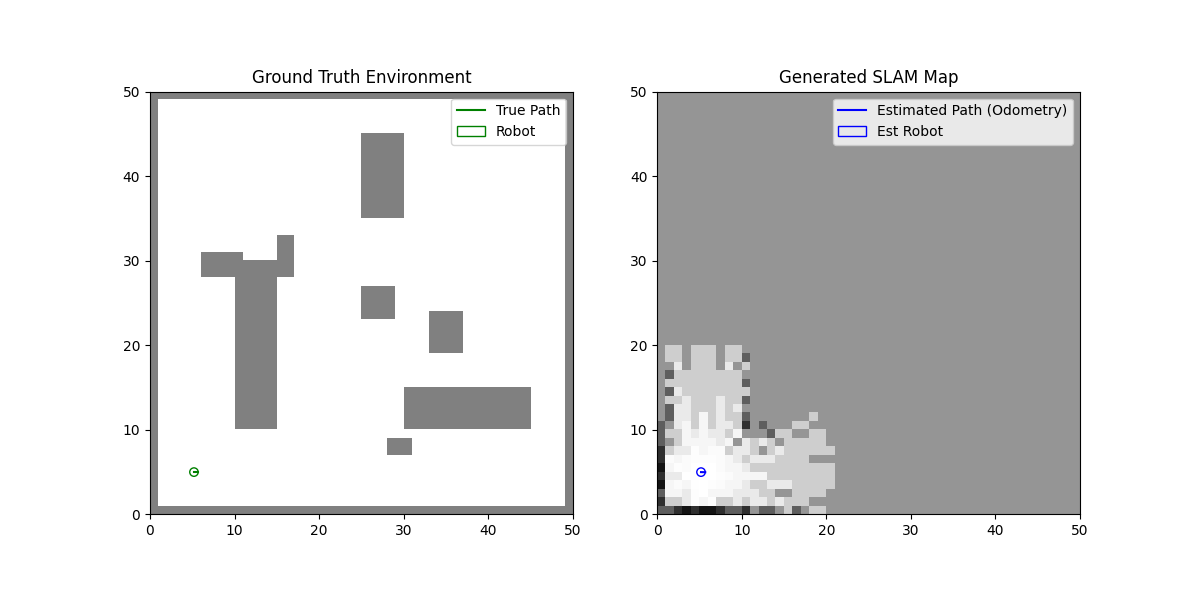
\includegraphics[width=0.95\textwidth]{plots/step_0000.png}
    \caption{Initial state (Step 0). The robot is at position (5, 5) with an empty occupancy grid.}
    \label{fig:step0}
\end{figure}

\begin{figure}[H]
    \centering
    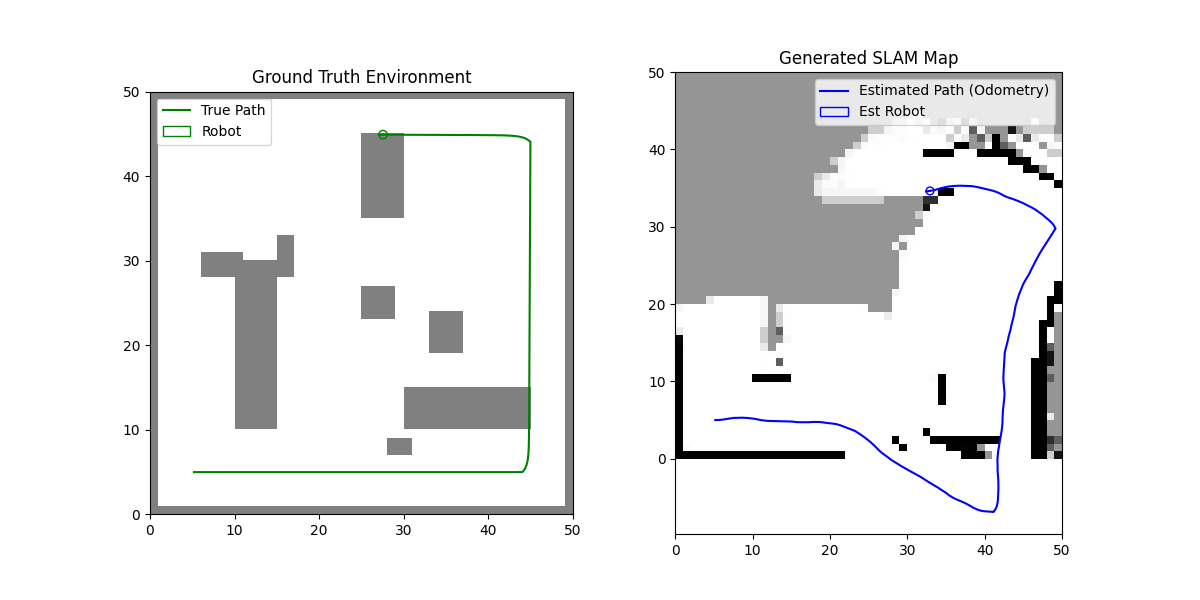
\includegraphics[width=0.95\textwidth]{plots/step_0500.png}
    \caption{Mid-exploration (Step 500). The occupancy grid shows partially reconstructed walls with visible distortion from accumulated odometry drift.}
    \label{fig:step500}
\end{figure}

\begin{figure}[H]
    \centering
    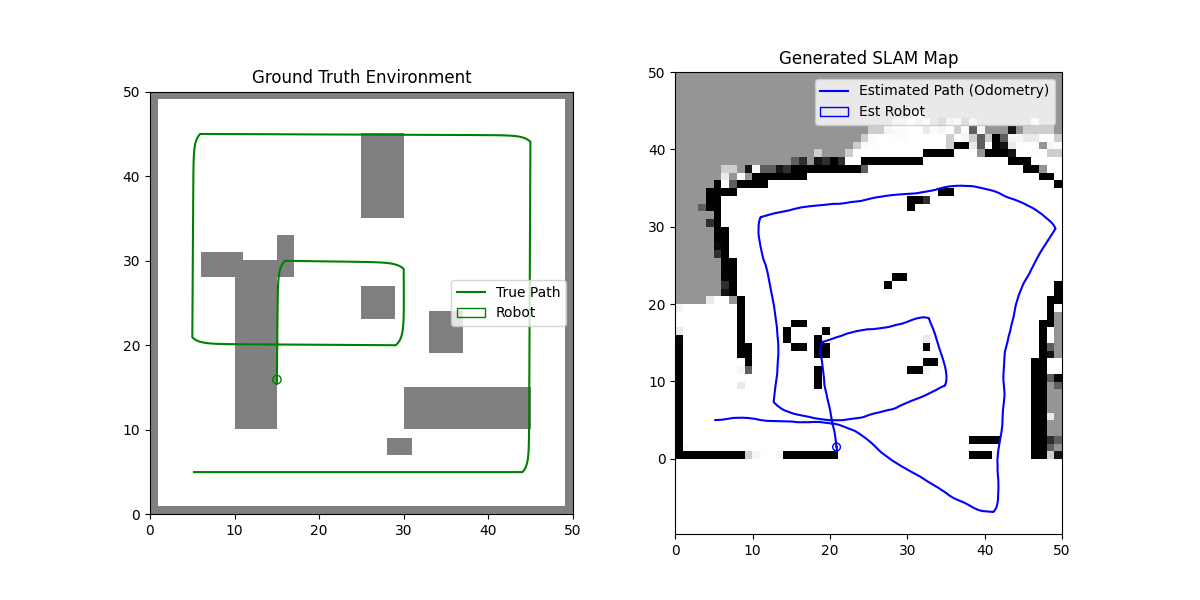
\includegraphics[width=0.95\textwidth]{plots/final_map.png}
    \caption{Final state (Step 1095). Left: true environment and true path (green). Right: SLAM-generated occupancy grid with estimated path (blue). Note the progressive divergence between the two paths due to odometry drift.}
    \label{fig:final}
\end{figure}

\subsection{Quantitative Evaluation}

The localisation error is measured as the \textbf{Mean Squared Error} between the true and estimated positions over all time steps:

\begin{equation}
    \text{MSE} = \frac{1}{T}\sum_{t=1}^{T}\left[(x_t - \hat{x}_t)^2 + (y_t - \hat{y}_t)^2\right]
\end{equation}

The simulation reports this at completion, providing a single scalar metric of odometry drift severity. By design---without any pose-correction mechanism (e.g., scan matching, loop closure)---this error is expected to grow monotonically, demonstrating the fundamental insufficiency of dead-reckoning alone.

\subsection{Qualitative Observations}

\begin{table}[H]
\centering
\begin{tabular}{@{}p{4.5cm}p{9cm}@{}}
\toprule
\textbf{Observation} & \textbf{Analysis} \\
\midrule
Wall structure is recognisable & Despite odometry drift, the log-odds formulation accumulates sufficient evidence to reveal major structures (boundaries, large obstacles). \\[4pt]
Map distortion increases with distance & The estimated path diverges progressively from the true path, causing later map updates to project rays from incorrect positions. This manifests as ``smeared'' or ``doubled'' walls in the occupancy grid. \\[4pt]
Small obstacles are less reliably mapped & Random blocks observed from only a few poses accumulate fewer log-odds updates and may appear faint or misaligned. \\[4pt]
Free-space mapping is robust & The Bresenham ray-tracing ensures that corridors the robot traverses are reliably marked as free, even with moderate pose error. \\
\bottomrule
\end{tabular}
\end{table}

% ══════════════════════════════════════════════════════════════
\section{Critical Analysis}

\subsection{Strengths}

\begin{enumerate}
    \item \textbf{Full-stack implementation:} Every component---kinematics, sensing, mapping, control, visualisation---is implemented from first principles, providing deep understanding of the SLAM pipeline.
    \item \textbf{Physically principled noise model:} The velocity-dependent odometry noise (\(\alpha_1\)--\(\alpha_4\)) is the standard model from probabilistic robotics, not an ad-hoc approximation.
    \item \textbf{Correct sensor--map separation:} LiDAR reads from the true world but maps using the estimated pose, faithfully replicating the real-world information flow.
    \item \textbf{Reproducibility:} Fixed random seed (42) ensures deterministic results.
    \item \textbf{Dual visualisation:} Simultaneous ground-truth and estimated-map display makes odometry drift immediately visible and pedagogically valuable.
\end{enumerate}

\subsection{Limitations}

\begin{enumerate}
    \item \textbf{No pose correction (open-loop SLAM):} The system performs \emph{mapping with odometry} but lacks the ``simultaneous localisation'' half of SLAM---there is no mechanism to correct the estimated pose using map observations. This means localisation error grows unboundedly.

    \item \textbf{No log-odds clamping:} Cells can saturate to extreme values (\(l \to \pm\infty\)), which could cause numerical issues in extended runs and prevents adaptation to dynamic environments.

    \item \textbf{Ray-casting resolution:} The 0.5\,m step size for LiDAR ray-casting can miss thin obstacles ($< 0.5$\,m). A smaller step or analytical ray--cell intersection would improve accuracy.

    \item \textbf{Fixed exploration path:} The predefined waypoints do not adapt to the discovered map. An information-theoretic exploration strategy (e.g., frontier-based exploration) would improve coverage efficiency.

    \item \textbf{No uncertainty representation for the pose:} The estimated pose is a single point estimate with no associated covariance, preventing the use of probabilistic fusion techniques (EKF, particle filters).

    \item \textbf{Variable shadowing in \texttt{slam.py}:} The loop variable \texttt{i} in the \texttt{update} method shadows the outer loop variable, which is a minor code quality issue.
\end{enumerate}

\subsection{Comparison with Full SLAM Solutions}

\begin{table}[H]
\centering
\small
\begin{tabular}{@{}p{2.8cm}p{2.5cm}p{2.5cm}p{2.8cm}p{2.8cm}@{}}
\toprule
\textbf{Feature} & \textbf{This Project} & \textbf{EKF-SLAM} & \textbf{FastSLAM} & \textbf{Graph-SLAM} \\
\midrule
Pose representation & Point estimate & Gaussian (\(\mu, \Sigma\)) & Particle set & Factor graph node \\[3pt]
Map representation & Occupancy grid & Landmark-based & Grid per particle & Occupancy grid \\[3pt]
Pose correction & None & Kalman update & Particle reweighting & Graph optimisation \\[3pt]
Loop closure & No & Limited & Yes (scan matching) & Yes (explicit) \\[3pt]
Scalability & \(O(n)\) per ray & \(O(n^2)\) landmarks & \(O(M \cdot K)\) & \(O(n^3)\) optimisation \\
\bottomrule
\end{tabular}
\end{table}

% ══════════════════════════════════════════════════════════════
\section{Future Work \& Extensions}

\subsection{Immediate Improvements}

\begin{enumerate}
    \item \textbf{Scan Matching (ICP / Correlative):} Aligning consecutive LiDAR scans to correct the estimated pose would dramatically reduce drift. The Iterative Closest Point (ICP) algorithm or Olson's correlative scan matching could be integrated with minimal architectural changes.

    \item \textbf{Log-Odds Clamping:} Adding bounds (e.g., \(l \in [-5, 5]\)) would prevent numerical saturation and allow the map to adapt if obstacles are moved.

    \item \textbf{Extended Kalman Filter (EKF) Integration:} Augmenting the \texttt{Robot} class with a state covariance matrix and implementing the EKF prediction/update cycle would provide principled pose uncertainty tracking.
\end{enumerate}

\subsection{Advanced Extensions}

\begin{enumerate}[resume]
    \item \textbf{Particle Filter (FastSLAM):} Maintaining \(M\) pose hypotheses, each with its own occupancy grid, would provide a complete probabilistic SLAM solution. The existing \texttt{OccupancyGridMap} class could be instantiated per particle with minimal modification.

    \item \textbf{Frontier-Based Exploration:} Replacing the fixed waypoint list with an autonomous exploration strategy that targets the boundaries between known-free and unknown space would enable full autonomous mapping.

    \item \textbf{Loop Closure Detection:} When the robot revisits a previously mapped area, detecting the match (e.g., via scan correlation) and correcting the accumulated drift would complete the SLAM pipeline.

    \item \textbf{3D Extension:} Extending the 2D grid to a 3D voxel representation (or using OctoMap) and replacing 2D LiDAR with a 3D point cloud would bring the system closer to real-world robotic applications.
\end{enumerate}

% ══════════════════════════════════════════════════════════════
\section{Repository Structure}

\begin{verbatim}
Msc/Robotics/
├── environment.py          # World model and LiDAR simulation
├── robot.py                # Differential-drive kinematics + odometry noise
├── slam.py                 # Log-odds occupancy grid with Bresenham
├── main.py                 # Simulation loop, controller, visualisation
├── visualization.html      # Interactive browser-based demo
├── plots/                  # Generated simulation snapshots
│   ├── step_0000.png ... step_1095.png
│   └── final_map.png
├── pyproject.toml          # uv project config (numpy, matplotlib)
└── README.md
\end{verbatim}

% ══════════════════════════════════════════════════════════════
\section{Conclusion}

This project demonstrates a working occupancy grid mapping system driven by simulated differential-drive kinematics and LiDAR sensing. The implementation successfully constructs a recognisable map of the environment, clearly illustrating both the power of the log-odds Bayesian update and the limitations of pure dead-reckoning localisation. The progressive degradation of map quality due to uncorrected odometry drift provides a compelling, visual motivation for the pose-correction mechanisms (scan matching, particle filters, graph optimisation) that distinguish full SLAM from mere mapping.

The codebase is modular, well-documented, and ready for extension---the most impactful next step would be integrating scan matching to close the localisation loop and transform this from an open-loop mapping system into a true SLAM solution.

% ══════════════════════════════════════════════════════════════
\section*{References}

\begin{enumerate}
    \item Thrun, S., Burgard, W. and Fox, D. (2005) \emph{Probabilistic Robotics}. MIT Press.
    \item Smith, R., Self, M. and Cheeseman, P. (1990) `Estimating Uncertain Spatial Relationships in Robotics', in Cox, I.J. and Wilfong, G.T. (eds.) \emph{Autonomous Robot Vehicles}. Springer, pp.~167--193.
    \item Elfes, A. (1989) `Using occupancy grids for mobile robot perception and navigation', \emph{Computer}, 22(6), pp.~46--57.
    \item Bresenham, J.E. (1965) `Algorithm for computer control of a digital plotter', \emph{IBM Systems Journal}, 4(1), pp.~25--30.
    \item Grisetti, G., Stachniss, C. and Burgard, W. (2007) `Improved Techniques for Grid Mapping With Rao-Blackwellized Particle Filters', \emph{IEEE Transactions on Robotics}, 23(1), pp.~34--46.
    \item Olson, E.B. (2009) `Real-time correlative scan matching', \emph{2009 IEEE International Conference on Robotics and Automation}, pp.~4387--4393.
\end{enumerate}

\end{document}
